

\tikzset{every picture/.style={line width=0.75pt}} %set default line width to 0.75pt        

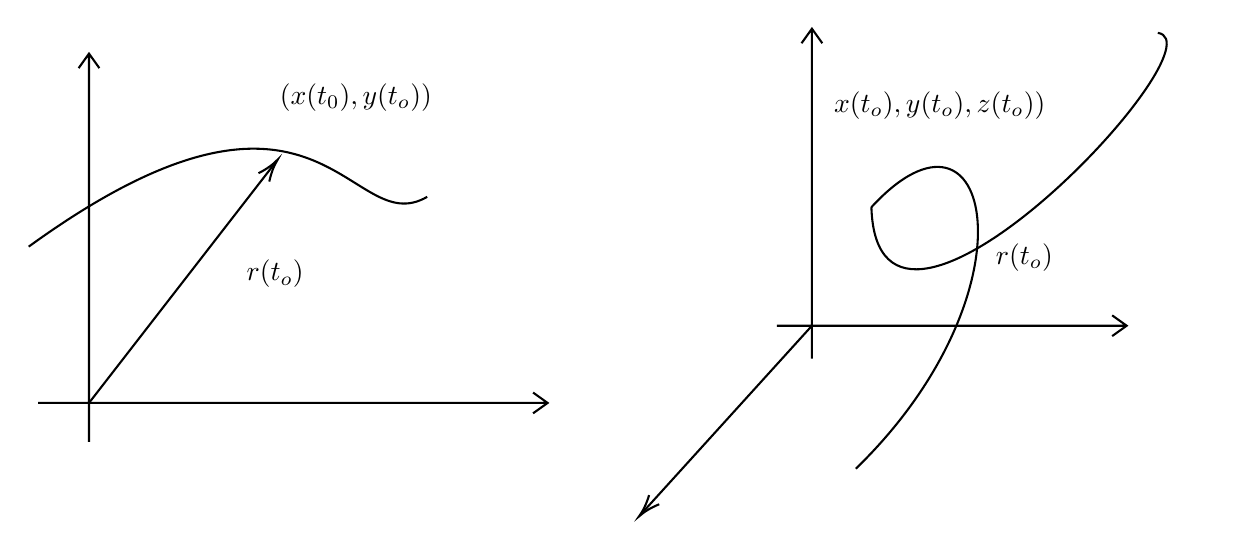
\begin{tikzpicture}[x=0.75pt,y=0.75pt,yscale=-1,xscale=1]
%uncomment if require: \path (0,310); %set diagram left start at 0, and has height of 310

%Shape: Axis 2D [id:dp34825501509521994] 
\draw  (23,212.3) -- (268.5,212.3)(47.55,44) -- (47.55,231) (261.5,207.3) -- (268.5,212.3) -- (261.5,217.3) (42.55,51) -- (47.55,44) -- (52.55,51)  ;
%Straight Lines [id:da7120917074211834] 
\draw    (47.55,212.3) -- (137.27,96.58) ;
\draw [shift={(138.5,95)}, rotate = 487.79] [color={rgb, 255:red, 0; green, 0; blue, 0 }  ][line width=0.75]    (10.93,-3.29) .. controls (6.95,-1.4) and (3.31,-0.3) .. (0,0) .. controls (3.31,0.3) and (6.95,1.4) .. (10.93,3.29)   ;
%Curve Lines [id:da9112376831548035] 
\draw    (18.5,137) .. controls (160.5,34) and (172.5,135) .. (210.5,113) ;
%Shape: Axis 2D [id:dp7523057169401708] 
\draw  (379,175.1) -- (547.5,175.1)(395.85,32) -- (395.85,191) (540.5,170.1) -- (547.5,175.1) -- (540.5,180.1) (390.85,39) -- (395.85,32) -- (400.85,39)  ;
%Straight Lines [id:da25097728151684107] 
\draw    (395.85,175.1) -- (313.84,265.52) ;
\draw [shift={(312.5,267)}, rotate = 312.21000000000004] [color={rgb, 255:red, 0; green, 0; blue, 0 }  ][line width=0.75]    (10.93,-3.29) .. controls (6.95,-1.4) and (3.31,-0.3) .. (0,0) .. controls (3.31,0.3) and (6.95,1.4) .. (10.93,3.29)   ;
%Curve Lines [id:da48745085294216717] 
\draw    (417,244) .. controls (505.5,158) and (482.5,55) .. (424.5,118) ;
%Curve Lines [id:da11758926162301764] 
\draw    (562.5,34) .. controls (595.5,39) and (427.5,217) .. (424.5,118) ;

% Text Node
\draw (138,57) node [anchor=north west][inner sep=0.75pt]    {$( x( t_{0}) ,y( t_{o}))$};
% Text Node
\draw (122,142) node [anchor=north west][inner sep=0.75pt]    {$r( t_{o})$};
% Text Node
\draw (405,61) node [anchor=north west][inner sep=0.75pt]    {$x( t_{o}) ,y( t_{o}) ,z( t_{o}))$};
% Text Node
\draw (483,134) node [anchor=north west][inner sep=0.75pt]    {$r( t_{o})$};


\end{tikzpicture}
